\documentclass[conference]{IEEEtran}
\IEEEoverridecommandlockouts
\usepackage{cite}
\usepackage{amsmath,amssymb,amsfonts}
\usepackage{algorithmic}
\usepackage{graphicx}
\usepackage{textcomp}
\usepackage{xcolor}
\usepackage{lipsum}
\usepackage{blindtext}
\usepackage{subfig}
\usepackage{caption}
\usepackage{placeins}
\usepackage{afterpage}
\usepackage{xurl}
\usepackage{gensymb}
\usepackage{stmaryrd}
\graphicspath{{./images/}}

\def\BibTeX{{\rm B\kern-.05em{\sc i\kern-.025em b}\kern-.08em
    T\kern-.1667em\lower.7ex\hbox{E}\kern-.125emX}}

\begin{document}

\title{Deep Reinforcement Learning with the MuJoCo Physics Simulator}

\author{
    \IEEEauthorblockN{Curtis Brinker}
    \IEEEauthorblockA{cjbzfd@mst.edu}
    \and
    \IEEEauthorblockN{Tanner May}
    \IEEEauthorblockA{tmay@mst.edu}
}
\maketitle

\begin{abstract}
    \blindtext
\end{abstract}

\section{Introduction}

Recent developments in machine learning have made huge strides in approaching problems that were previously unsolvable
with traditional programming methods. In general, machine learning techniques are grouped into three categories:
supervised learning, unsupervised learning, and reinforcement learning (RL) \cite{rl_application}.

\blindtext
\blinditemize[4]

\blindtext

\section{Testing Environment}

Each of the models were trained using Open AI's Gym library and DeepMind's physics simulator MuJoCo. The Gym toolkit
implements numerous environments for testing RL, such as the MuJoCo physics simulator. MuJoCo stands
for {\bf Mu}lti-{\bf Jo}int dynamics with {\bf Co}ntact and was made for applications that require fast, accurate
physics simulations such as robotics and machine learning \cite{mujoco_docs}. Using MuJoCo, machine learning
algorithms can learn how to control the movement of robotic models, such as a snake, ant, or humanoid.

Each of the Gym's environments adhere to a strict structure that makes it easy to switch between environments. One of
the most important parts to keep consistent are the values returned after every step of training. Each environment
returns the following four values \cite{gym_docs}:

\begin{itemize}
    \item Observation: Represents the current state of the environment, as the agent sees it. In MuJoCo's case, the
    environment is fully observable and consists of the model's position, velocity, and various forces \cite{gym_source}
    \item Reward: The reward result of the previous action. The reward for the MuJoCo environment depends on a
    number of things and is unique for each model.
    \item Done: A flag denoting if the environment needs to be reset. Each of the models in MuJoCo define a safe height
    range that the model is allowed to exist within; if the model leaves that range, the done flag is raised and the
    model is reset back to the start.
    \item Info: Some information useful for debugging.
\end{itemize}



<Some sort of final words and transition into the background section.>

\section{Background}

\blindtext

\subsection{Advantage Actor Critic (A2C)}

\blindtext

\subsection{Deep Deterministic Policy Gradient (DDPG)}

\blindtext

\subsection{Soft Actor Critic (SAC)}

\blindtext

\section{Methodology}

Each of the algorithms were implemented on Ubuntu 20.04 with Python 3.8 using the PyTorch library. We used PyTorch
because we had previous experience with it and liked how flexible it is compared to other options. To train the models,
we used the previously mentioned Gym library. To verify that the implementation of each of the algorithms worked
correctly, we trained them using the Pendulum-v1 environment whose goal is to simply swing a pendulum so it stays
upright. For training towards our goal, we used the MuJoCo environment with the Ant-v3 and Humanoid-v3 models. The ant
model was chosen because it is relatively simple (four legs, two joints each) and will still teach the algorithm to walk
in a three dimensional environment. The humanoid model was chosen because it is significantly more complex (two legs and
a total of seventeen joints) and should showcase the learning power of the algorithms.

Since the models have vastly different complexities the amount of training steps varied between them, but not between RL
algorithms. Each of the algorithms was able to train with the ant model for 500,000 steps; after 500,000 steps, training
was stopped and the most recently saved model was used. We chose 500,000 steps since it seemed to produce good results
(a model that moved a non-trivial distance) for all of the algorithms tested. Training with the humanoid model was
conducted for 1,250,000 steps. But, since training took so long, we only trained the SAC algorithm because it produced
the most interesting results during the ant training phase.

The hyperparameters for each algorithm were as follows:
\begin{itemize}
    \item A2C: Learning rate of $3e^{-4}$ and $\gamma = 0.99$.
    \item DDPG: Update freq. of 64 steps, update threshold of 4096 steps, batch size of 128, learning rate of $1e^{-3}$,
    $\gamma = 0.99$, $\tau = 0.995$, and the noise distribution was Normal with a standard deviation of 0.1.
    \item SAC: Update freq. of 64 steps, 64 updates per update step, an update threshold of 4096 steps, batch size of
    128, $\alpha = 0.5$, learning rate of $5e^{-4}$, $\gamma = 0.99$, $\tau = 0.995$, and an $\alpha$ decay of 1.
\end{itemize}
Each of those parameters were chosen because they resulted in the best performing model.

Since our goal is to teach Deep RL algorithms how to walk, we defined the networks for each of the algorithms to have
two layers, each with 256 neurons. Originally we tried 128 neurons each but algorithms using the 256 neuron
configuration had better performance. More layers and neurons can, of course, be used but would have greatly increased
the computational cost of training.

Since every environment has its own quirks, each is described in its own subsection below \cite {gym_source}.

\subsection{CartPole-v0}

<image of cartpole?>
The objective of the CartPole environment is to teach an agent to balance a pole on a cart by moving the cart left and
right. The environment has a continuous observation space consisting of the cart's position, the cart's velocity, the
pole's angle, and the pole's angular velocity. The action space is discrete with the options of moving the cart to the
left or to the right. The environment rewards the agent with a value of one, simply for staying healthy.

Initially, the values of both the cart and pole are randomly sampled from a uniform distribution from $[-0.5, 0.5]$. The
environment is terminated when the angle of the pole is $\pm12\degree$, the cart position hits the edge of the display,
or when the length of the episode surpasses 200 steps. The environment is considered solved when the reward is
\textgreater 195 for 100 consecutive episodes.

This environment was used as a proof of concept of each algorithm's implementation.

\subsection{Pendulum-v1}

<image of pendulum?>
The pendulum environment's objective is to balance a frictionless pendulum straight up. The observation space is
continuous and describes the angle of the pendulum as well as the angular velocity. The action space is also continuous
and details the amount of left or right force to apply to the pendulum. The reward incentivises keeping the pole at an
angle of $0\degree$ with as little velocity and force as possible. The reward is formulated as
$$
R = -(angle ^{2} + 0.1 * angular\_velocity ^ {2} + 0.001 * action ^ {2})
$$
Since the angle is normalized between $[-\pi, \pi]$ before calculating the reward, the reward has a range of
$[-16.3, 0]$.

The environment's initial state has the pole at a random angle between $[-\pi, \pi]$ radians with a random velocity
between $[-1, 1]$. The environment does not specify a termination state, so a limit of 150 was imposed. Similarly, the
environment does not specify when it is solved, so it was allowed to run until it hit the step limit.

Like the CartPole environment, this environment was used as another proof of concept of the implementation for each
algorithm.

\subsection{Ant-v3}

<image of ant?>
The ant is a sphere with four legs, each with two joints. The continuous observation space is significantly more
complex than the previous environments: it consists of the model's position, velocity, and the forces between the legs
and the ground (contact force). The action space is also continuous and describes where and how quickly to move each
joint. The reward encourages the model to move as quickly as possible while moving as few joints as little and softly as
possible. It is formulated as
$$
R = (v + h) - (a + f)
$$
where $v$ is the velocity in the x-axis, $h$ is the healthy reward configured to be 1, $a$ is the control\_cost
calculated by $0.5* \sum actions^{2}$, and $f$ is the contact\_cost calculated by
$5e^{-4} * \sum contact\_forces^{2}$.

The environment starts with each joint in a random position with a random velocity. The episode is terminated when the
model exits the safe height range of $[0.3, 2.0]$. The environment did not define a solve condition so the episode was
continued until the model made a mistake to trigger the termination condition.

The ant was chosen because it is the simplest provided model that meets the "three dimensional walker" condition.

\subsection{Humanoid-v3}

<image of humanoid?>
The humanoid model is a humanoid with two legs, two arms, a head and a torso. The legs, arms, and torso are made up of
multiple joints, each individually controlled. Like the ant, the observation space is continuous and describes the
model's position, the model's velocity, the forces for each of the joints, and the contact forces. The environment also
defines a continuous action space that describes the new position and velocity of each joint. The intution for the
reward is the same as for the Ant environment, but it is calculated slightly differently where $v$ is equal to
$1.25 * x\_velocity$, $h$ is configured to be 5, $a$ is calculated as $0.1 * \sum actions^{2}$, and $f$ is defined as
$5e^{-7} * \sum contact\_forces^{2}$.

Like the Ant environment, the model starts with each joint in a random position and random velocity. The episode is
terminated when the model exits the safe height range of $[1.0, 2.0]$. The environment did not define a solve condition
so the episode was continued until the model made a mistake to trigger the termination condition.

The humanoid was chosen because it is the most complex 3D walker and should showcase the learning power of the tested
algorithms.

\section{Results}

\blindtext

\subsection{CartPole-v0}

\blindtext

\subsection{Pendulum-v1}

\begin{figure}
    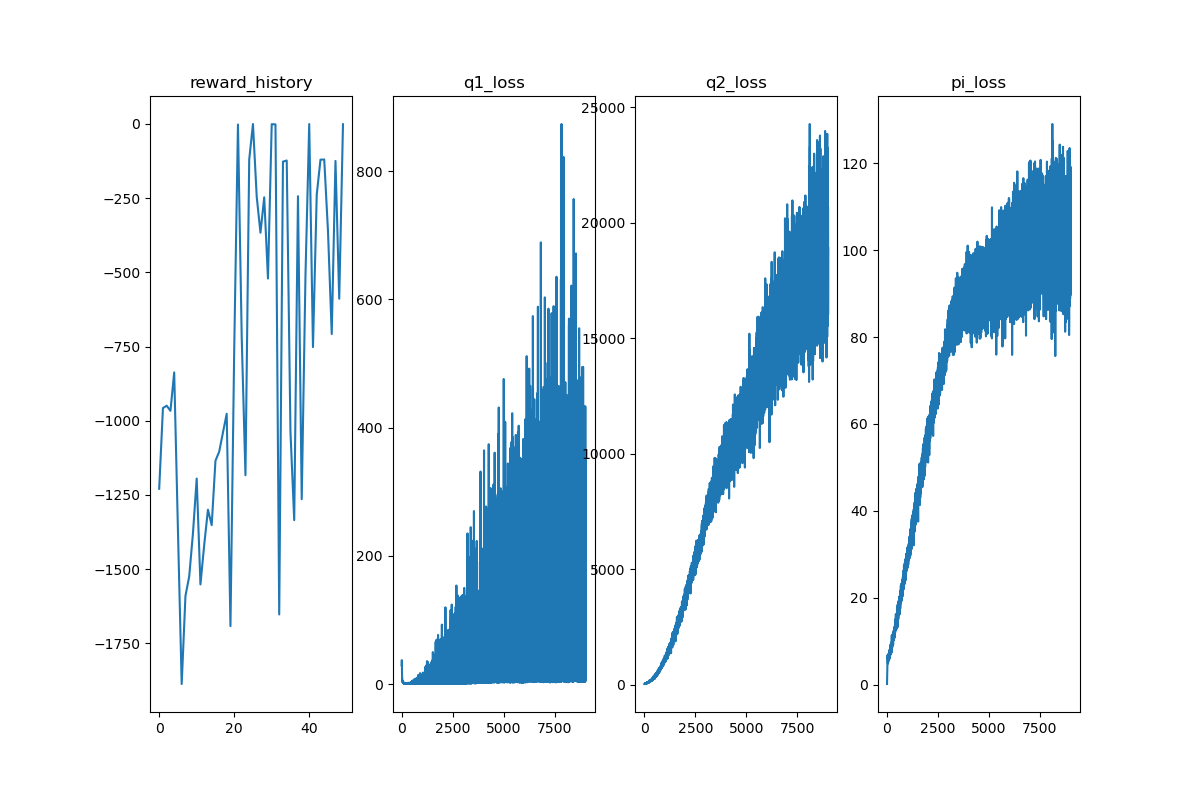
\includegraphics[width=0.45\textwidth]{sac-pendulum}
    \caption{SAC in the Pendulum-v1 Environment}
\end{figure}

\blindtext

\subsection{Ant-v3}

\begin{figure}
    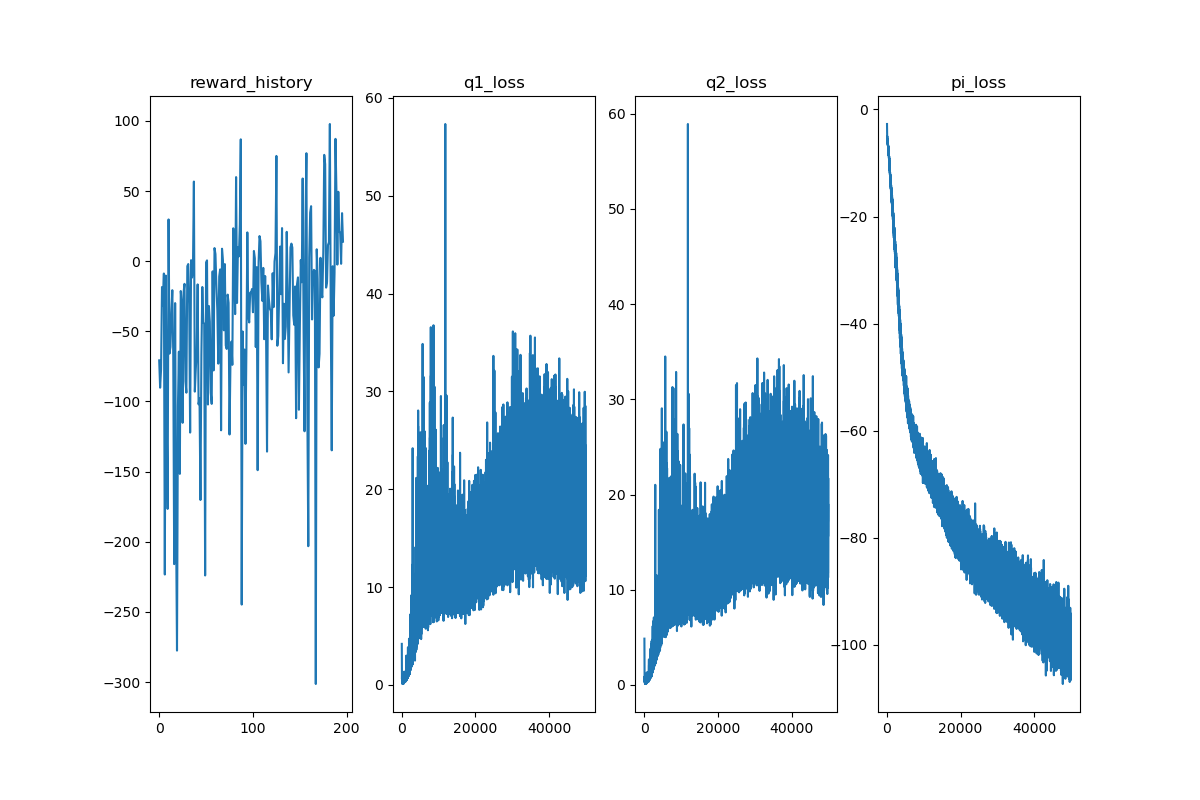
\includegraphics[width=0.45\textwidth, height=5cm]{sac-ant}
    \caption{SAC in the Ant-v3 environment}
\end{figure}

\begin{figure}
    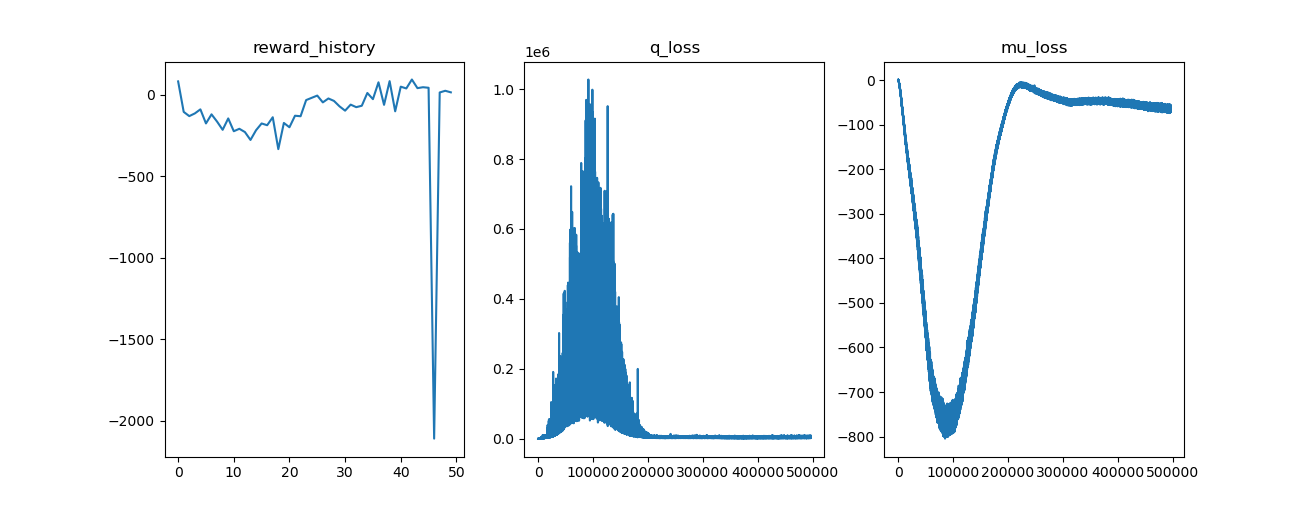
\includegraphics[width=0.45\textwidth, height=5cm]{ddpg-ant}
    \caption{DDPG in the Ant-v3 environment}
\end{figure}

\blindtext

\subsection{Humanoid-v3}

\blindtext

\section{Future Work and Conclusions}

\blindtext[2]


\bibliography{references}
\bibliographystyle{ieeetran}


\end{document}
